\documentclass[a4paper,sigconf]{acmart}
%DIF LATEXDIFF DIFFERENCE FILE
%DIF DEL Publication_old\main.tex   Thu Jan 25 16:14:46 2024
%DIF ADD Publication\main.tex       Fri Jan 26 19:15:06 2024
\usepackage{hyperref}
\usepackage{cleveref}
\usepackage{tikz}
\usepackage{tcolorbox}
%DIF 6d6
%DIF < \usepackage{todonotes}
%DIF -------
\title{Prompt Injection Attacks against LLMs}
\setcopyright{rightsretained}
\copyrightyear{2024}
\acmYear{2024}
\acmDOI{}
\acmConference[HoT-MLSEC Conference 2024]{HoT-MLSEC Conference 2024}{February 16, 2024}{KIT, Karlsruhe, Germany}
\acmBooktitle{Proceedings of HoT-MLSEC Conference 2024,
February 16, 2024, KIT, Karlsruhe, Germany}
\acmISBN{}
\settopmatter{printacmref=false}
\settopmatter{printccs=false}
\keywords{Prompt Injection, LLM, Cybersecurity, SoK} % <--- Set keywords that match your topic!
\geometry{twoside=true, head=13pt, paperwidth=210mm, paperheight=297mm, includeheadfoot, columnsep=2pc, top=57pt, bottom=73pt, inner=54pt, outer=54pt,  marginparwidth=2pc,heightrounded  } %DIF > 
%DIF PREAMBLE EXTENSION ADDED BY LATEXDIFF
%DIF UNDERLINE PREAMBLE %DIF PREAMBLE
\RequirePackage[normalem]{ulem} %DIF PREAMBLE
\RequirePackage{color}\definecolor{RED}{rgb}{1,0,0}\definecolor{BLUE}{rgb}{0,0,1} %DIF PREAMBLE
\providecommand{\DIFaddtex}[1]{{\protect\color{blue}\uwave{#1}}} %DIF PREAMBLE
\providecommand{\DIFdeltex}[1]{{\protect\color{red}\sout{#1}}}                      %DIF PREAMBLE
%DIF SAFE PREAMBLE %DIF PREAMBLE
\providecommand{\DIFaddbegin}{} %DIF PREAMBLE
\providecommand{\DIFaddend}{} %DIF PREAMBLE
\providecommand{\DIFdelbegin}{} %DIF PREAMBLE
\providecommand{\DIFdelend}{} %DIF PREAMBLE
\providecommand{\DIFmodbegin}{} %DIF PREAMBLE
\providecommand{\DIFmodend}{} %DIF PREAMBLE
%DIF FLOATSAFE PREAMBLE %DIF PREAMBLE
\providecommand{\DIFaddFL}[1]{\DIFadd{#1}} %DIF PREAMBLE
\providecommand{\DIFdelFL}[1]{\DIFdel{#1}} %DIF PREAMBLE
\providecommand{\DIFaddbeginFL}{} %DIF PREAMBLE
\providecommand{\DIFaddendFL}{} %DIF PREAMBLE
\providecommand{\DIFdelbeginFL}{} %DIF PREAMBLE
\providecommand{\DIFdelendFL}{} %DIF PREAMBLE
%DIF HYPERREF PREAMBLE %DIF PREAMBLE
\providecommand{\DIFadd}[1]{\texorpdfstring{\DIFaddtex{#1}}{#1}} %DIF PREAMBLE
\providecommand{\DIFdel}[1]{\texorpdfstring{\DIFdeltex{#1}}{}} %DIF PREAMBLE
%DIF COLORLISTINGS PREAMBLE %DIF PREAMBLE
\RequirePackage{listings} %DIF PREAMBLE
\RequirePackage{color} %DIF PREAMBLE
\lstdefinelanguage{DIFcode}{ %DIF PREAMBLE
%DIF DIFCODE_UNDERLINE %DIF PREAMBLE
  moredelim=[il][\color{red}\sout]{\%DIF\ <\ }, %DIF PREAMBLE
  moredelim=[il][\color{blue}\uwave]{\%DIF\ >\ } %DIF PREAMBLE
} %DIF PREAMBLE
\lstdefinestyle{DIFverbatimstyle}{ %DIF PREAMBLE
	language=DIFcode, %DIF PREAMBLE
	basicstyle=\ttfamily, %DIF PREAMBLE
	columns=fullflexible, %DIF PREAMBLE
	keepspaces=true %DIF PREAMBLE
} %DIF PREAMBLE
\lstnewenvironment{DIFverbatim}{\lstset{style=DIFverbatimstyle}}{} %DIF PREAMBLE
\lstnewenvironment{DIFverbatim*}{\lstset{style=DIFverbatimstyle,showspaces=true}}{} %DIF PREAMBLE
%DIF END PREAMBLE EXTENSION ADDED BY LATEXDIFF

\begin{document}
\author{Denis Wambold}
\email{denis.wambold@student.kit.edu}
\affiliation{%
  \institution{Karlsruhe Institute of Technology}
  \city{Karlsruhe}
  \country{Germany}
}

\begin{abstract}
Large Language Models (LLMs) have gained huge popularity in recent years. 
\DIFdelbegin \DIFdel{Not only for scientific usage and research, but also for the everyday usage of millions of people. 
}\DIFdelend Being widely available to the public, these Natural Language Processing \DIFdelbegin \DIFdel{Models are able to }\DIFdelend \DIFaddbegin \DIFadd{models can }\DIFaddend answer human-written input prompts with output prompts hard to distinguish from human-written answers.
Since so many people use LLMs \DIFdelbegin \DIFdel{on a dailybasis}\DIFdelend \DIFaddbegin \DIFadd{daily}\DIFaddend , they can carry sensitive user data or be used to trick benign users.
Thus, they also attract the attention of adversaries, who are interested in sensitive data, causing damage to the \DIFdelbegin \DIFdel{Model }\DIFdelend \DIFaddbegin \DIFadd{model }\DIFaddend or benign users, or simply love chaos.
\DIFdelbegin %DIFDELCMD < 

%DIFDELCMD < %%%
\DIFdel{Currently, there are many known attacks against LLMs. 
However, almost all of them are new, and seemingly no benign users know of their existence of how to handle them.
For them, prompt injection attacks are especially dangerous. 
On top of that}\DIFdelend \DIFaddbegin \DIFadd{A straightforward way to attack a LLM is the so called prompt injection which attacks the LLM with user-given input. 
Currently}\DIFaddend , there is a lack of categorization \DIFdelbegin \DIFdel{of those}\DIFdelend \DIFaddbegin \DIFadd{for these types of attacks}\DIFaddend . 
Without a categorization\DIFdelbegin \DIFdel{of attacks}\DIFdelend , it is hard to prevent \DIFdelbegin \DIFdel{them }\DIFdelend \DIFaddbegin \DIFadd{attacks }\DIFaddend on a wide scale or implement countermeasures.
\DIFdelbegin %DIFDELCMD < 

%DIFDELCMD < %%%
\DIFdelend Hence, in this paper, we introduce a taxonomy for prompt injection attacks against LLMs.
To do so, we analyze \DIFdelbegin \DIFdel{well known }\DIFdelend \DIFaddbegin \DIFadd{well-known }\DIFaddend prompt injection attacks against LLMs and split the attacks into three fundamental parts: The attack vector, the mode of operation\DIFaddbegin \DIFadd{, }\DIFaddend and the goal of the attack. 
Then, we split each of those parts into multiple subcategories to allow a fine-grained categorization of attacks. 
Using our taxonomy, we achieve a wide coverage of (possible) prompt injection attacks against LLMs, allowing categorization and comparison.
Furthermore, we glance at possible defense mechanisms and discuss our taxonomy \DIFdelbegin \DIFdel{, }\DIFdelend to ensure the security of LLMs against prompt injection attacks.
\end{abstract}
\maketitle
\section{\textit{Introduction}}
Nowadays, \DIFdelbegin \DIFdel{Lange Language Models }\DIFdelend \DIFaddbegin \DIFadd{Large Language Models (LLMs) }\DIFaddend are omnipresent. \DIFdelbegin \DIFdel{Students, Research,  }\DIFdelend \DIFaddbegin \DIFadd{Used by students, in research,  or }\DIFaddend assisting everyday tasks\DIFdelbegin \DIFdel{. Seemingly }\DIFdelend \DIFaddbegin \DIFadd{, seemingly }\DIFaddend everyone uses them. 
This recently gained popularity makes them particularly attractive for adversaries. 
And since \DIFdelbegin \DIFdel{Large Language Models }\DIFdelend \DIFaddbegin \DIFadd{LLMs }\DIFaddend come in various forms, it seems like there is infinite room for the creativity of adversaries to attack them. 
One of the most versatile types of attacks are \DIFdelbegin \DIFdel{so called }\DIFdelend prompt injection attacks\DIFaddbegin \DIFadd{~\mbox{%DIFAUXCMD
\cite{10.1145/3605764.3623985}}\hskip0pt%DIFAUXCMD
}\DIFaddend , in which the adversary communicates with the LLM via prompts and instructions.

Since this recent uprise of \DIFdelbegin \DIFdel{Large Language Models is quite new }\DIFdelend \DIFaddbegin \DIFadd{LLMs is rather current }\DIFaddend and the models \DIFdelbegin \DIFdel{seem to evolving at superhuman speeds, }\DIFdelend \DIFaddbegin \DIFadd{evolve at rapid speeds, developing LLMs to be more robust against prompt injection attacks is now more important than ever. However, }\DIFaddend there is no taxonomy yet to categorize these \DIFdelbegin \DIFdel{prompt injection }\DIFdelend attacks. 
Therefore, it is especially hard to defend against them without tackling every single attack pattern one by one.
Finding similarities and \DIFdelbegin \DIFdel{and differences , }\DIFdelend \DIFaddbegin \DIFadd{differences and }\DIFaddend forming groups of attacks \DIFdelbegin \DIFdel{, enables }\DIFdelend \DIFaddbegin \DIFadd{allows }\DIFaddend developers to implement defense mechanisms \DIFdelbegin \DIFdel{and further develop models to be more robust against prompt injection attacks is now more important than ever}\DIFdelend \DIFaddbegin \DIFadd{more easily}\DIFaddend . 

We introduce a novel taxonomy, allowing a fine grained categorization of prompt injection attacks against \DIFdelbegin \DIFdel{Large Language Models}\DIFdelend \DIFaddbegin \DIFadd{LLMs}\DIFaddend . 
To achieve this, \DIFaddbegin \DIFadd{we }\DIFaddend split attacks along three axes: The attack vector, the mode of operation and the goal of the attack.
These three axes then are split into different (not necessarily disjoint) subcategories, resulting in a wide coverage of the field. 
Our main contributions are the following:

\begin{itemize}
    \item R1: \DIFdelbegin \DIFdel{Analyze }\DIFdelend \DIFaddbegin \DIFadd{We analyze }\DIFaddend the current state of the field and find similarities and differences among \DIFaddbegin \DIFadd{prompt injection }\DIFaddend attack patterns.
    \item R2: \DIFdelbegin \DIFdel{Use }\DIFdelend \DIFaddbegin \DIFadd{We use }\DIFaddend gained knowledge to present a taxonomy to categorize prompt injection attacks \DIFaddbegin \DIFadd{and introduce defense mechanisms}\DIFaddend .
    \item R3: \DIFdelbegin \DIFdel{Discuss }\DIFdelend \DIFaddbegin \DIFadd{We discuss the taxonomy and }\DIFaddend defense mechanisms for prompt \DIFdelbegin \DIFdel{injection attacks}\DIFdelend \DIFaddbegin \DIFadd{injections}\DIFaddend .
\end{itemize}

We start by introducing important background knowledge of the field needed to understand our taxonomy and the used attacks. 
After that, we introduce our taxonomy \DIFdelbegin \DIFdel{, where we not only }\DIFdelend \DIFaddbegin \DIFadd{and }\DIFaddend present the different categories we observed during our research\DIFdelbegin \DIFdel{, but also discuss a possible appropriate threat model}\DIFdelend .
Next, we briefly talk about the defense against prompt injection attacks and how to handle them properly.
Then, we discuss our taxonomy, the defense and give an outlook to what can further be researched.
Finally, \DIFaddbegin \DIFadd{we }\DIFaddend conclude the contributions of this paper.
\section{\textit{Background}}
In this section, we introduce the necessary background knowledge to understand the context of this paper. 
The explanation will be on a high level as going into detail for each topic would go beyond the scope of this work. 
For further information, please refer to the cited sources.

First, we introduce \DIFdelbegin \DIFdel{Large Language Models}\DIFdelend \DIFaddbegin \DIFadd{LLMs}\DIFaddend .
Then, we explain the general concept of prompt injection attacks against \DIFdelbegin \DIFdel{Large Language Models}\DIFdelend \DIFaddbegin \DIFadd{LLMs}\DIFaddend .
Finally, we \DIFdelbegin \DIFdel{explain so called jailbreak attacks}\DIFdelend \DIFaddbegin \DIFadd{discuss the usage of a threat model}\DIFaddend .
\subsection{\textit{Large Language Models}}
Large Language Models \DIFdelbegin \DIFdel{(LLMs) }\DIFdelend are a type of neural network.
More specifically, they are Natural Language Processing \DIFdelbegin \DIFdel{(NLP) }\DIFdelend models based on the Transformer \DIFdelbegin \DIFdel{Architecture}\DIFdelend \DIFaddbegin \DIFadd{architecture}\DIFaddend ~\cite{vaswani2023attention, floridi2020gpt, thoppilan2022lamda}.
\DIFaddbegin \DIFadd{This architecture is particularly effective when processing sequential data, like (long) texts. 
}\DIFaddend Therefore, they \DIFdelbegin \DIFdel{train }\DIFdelend \DIFaddbegin \DIFadd{can be trained }\DIFaddend to understand and predict human language patterns.
\DIFdelbegin \DIFdel{Consisting of billions of nodes, LLMs have the capability to }\DIFdelend \DIFaddbegin \DIFadd{LLMs fulfill this task. Equipped with billions of parameters, they }\DIFaddend train on large corpora of (text) data.
\DIFaddbegin \DIFadd{The training of LLMs can be split up into two distinct phases.
During the first phase, the pre-training, the model is trained to solve general tasks, like predicting the next word or context of a sentence~\mbox{%DIFAUXCMD
\cite{radford2018improving}}\hskip0pt%DIFAUXCMD
.
After that, during the fine-tuning phase, the LLM is fine-tuned to solve more specific tasks. 
Additionally, in the second step, the LLM can be configured and aligned with custom policies. 
This alignment is especially important, as it prevents the LLM from answering malicious prompts aiming to exploit it. 
For benign users, the alignment forces the LLM to stay as politically and ethically correct as possible.
}\DIFaddend Once fully trained, the LLM receives an input, called \textit{prompt}, and outputs a \textit{response}~\cite{floridi2020gpt, thoppilan2022lamda}.
Their vast size allows them to generate responses that are almost indistinguishable from human-written text.
In combination with their ability to generate \DIFdelbegin \DIFdel{text in a variety of }\DIFdelend \DIFaddbegin \DIFadd{texts of different }\DIFaddend styles, LLMs are used in a variety of applications, such as text generation, translation, summarizing, and question answering~\cite{floridi2020gpt, thoppilan2022lamda}.
\DIFaddbegin \DIFadd{However, this is to be enjoyed with care as the power of a LLM is not only attractive to normal users. 
Over time, the LLM is exposed to many risks. It can collect user-specific information that is very valuable to other malicious users or be exposed to external injected bias.
These two risks are only a few of many a LLM faces, which makes it even more important to secure it against evil intent.
}\DIFaddend 

Additionally, LLMs are not only useful for direct human interaction.
Recent development shows that they can also be integrated \DIFdelbegin \DIFdel{in }\DIFdelend \DIFaddbegin \DIFadd{into }\DIFaddend applications to offer interactive functionalities, oftentimes by calling external \DIFdelbegin \DIFdel{APIs}\DIFdelend \DIFaddbegin \DIFadd{Application Programming Interfaces (APIs)}\DIFaddend .
However, this does not come without security risks~\cite{10.1145/3605764.3623985, liu2023demystifying, pedro2023prompt}. 
Especially external connections and the rapidly growing, extensive, use of \DIFdelbegin \DIFdel{AI-functionality poses }\DIFdelend \DIFaddbegin \DIFadd{AI functionality pose }\DIFaddend a security risk to the application if not properly secured and monitored.
\subsection{\textit{Prompt Injection}}
Even the most powerful LLM renders useless without a prompt.
Most of the time, only the prompt enables the user to interact with the LLM and is the only way to control the output of the LLM.
Consequently, the prompt is a convenient way for a malicious user to take over or manipulate that response~\cite{perez2022ignore}.

We define prompt injection attacks as the malicious input of prompts to a LLM to manipulate the LLM itself or its response. 
\DIFaddbegin \DIFadd{A successful prompt injection can exploit the LLM without changing its state or performing prohibited actions.
If used properly, prompt injection attacks can therefore circumvent content restrictions, or even security filters, of the LLM.
This can not only lead to the leakage of sensitive information but also to the execution of malicious code or other unintended, potentially harmful, behavior.
}\DIFaddend Somewhat counterintuitively, input prompts are not always directly user-given, but can also be hidden in \DIFdelbegin \DIFdel{input-data }\DIFdelend \DIFaddbegin \DIFadd{input data }\DIFaddend or even in the data \DIFdelbegin \DIFdel{the LLM was trained on}\DIFdelend \DIFaddbegin \DIFadd{retrieved by the LLM}\DIFaddend ~\cite{10.1145/3605764.3623985}.
In the latter case, there is no clear line between data and prompts \DIFaddbegin \DIFadd{from the model side}\DIFaddend , which confuses the LLM and leads to unexpected behaviour~\cite{10.1145/3605764.3623985}.
\DIFdelbegin \DIFdel{If used properly, prompt injection attacks can circumvent content restrictions, or even securityfilters, of }\DIFdelend \DIFaddbegin \subsection{\textit{\DIFadd{Threat Model}}}
\DIFadd{In cyber security, the process of threat modeling is crucial for the analysis of }\DIFaddend the \DIFdelbegin \DIFdel{LLM.
This can not only lead to the leakage of sensitive information, but also to the execution of malicious code or other unintended, potentially harmful, behavior.
}\subsection{\textit{\DIFdel{Jailbreak Attacks}}%DIFAUXCMD
}
%DIFAUXCMD
\addtocounter{subsection}{-1}%DIFAUXCMD
\DIFdel{Jailbreak attacks are a special type of prompt injection attacks.
Due to }\DIFdelend \DIFaddbegin \DIFadd{security of systems.
A threat model helps to analyze potential attacks and understand the attacker's goals~\mbox{%DIFAUXCMD
\cite{XIONG201953}}\hskip0pt%DIFAUXCMD
.
Typically, these threat models are used to outline the possibilities of an adversary to get an overview of present risks.
}

\DIFadd{Prompt injection attacks are diverse and work very differently, as we show in our taxonomy. 
One single threat model cannot outline the different scenarios of attacks appropriately.
Therefore, we decided not to introduce a fixed threat model in this work and instead forward it to }\DIFaddend the \DIFdelbegin \DIFdel{large size of the data a LLM trains on, it is not possible to manually check all of it.
Hence, the data is not always clean and can contain malicious content, or content that could assist malicious activities.
Thus, many LLMs only work under restrictions and are configured to avoid some topics, to not output certain content or answer certain, malicious, prompts. 
If the LLM is not properly secured, it is be possible to trick the model into answering these, usually banned, prompts. This is achieved by carefully crafting special prompts, sometimes in an iterative manner, to test the boundaries of the LLM step by step~\mbox{%DIFAUXCMD
\cite{wei2023jailbroken, chao2023jailbreaking}}\hskip0pt%DIFAUXCMD
.
This process of circumventing built-in security mechanism is called a Jailbreak Attack, as the LLM is "breaking out of its jail" and answering prompts it is not supposed to answer}\DIFdelend \DIFaddbegin \DIFadd{original authors of the mentioned attacks, as most of them propose threat models themselves}\DIFaddend .
\section{\textit{Taxonomy}}
\label{taxonomy}
Prompt injection \DIFaddbegin \DIFadd{(PI) }\DIFaddend attacks come in various kinds and can be \DIFdelbegin \DIFdel{totally }\DIFdelend \DIFaddbegin \DIFadd{very }\DIFaddend different.
From something seemingly uninteresting, like making a model say a word it is not allowed to \cite{chao2023jailbreaking}, up to stealing sensitive data or injecting code \cite{10.1145/3605764.3623985}, there is no end \DIFdelbegin \DIFdel{for }\DIFdelend \DIFaddbegin \DIFadd{to }\DIFaddend the creativity of an adversary. 

To give a more manageable overview \DIFdelbegin \DIFdel{over }\DIFdelend \DIFaddbegin \DIFadd{of }\DIFaddend the field of \DIFdelbegin \DIFdel{prompt injection attacks against Large Language models}\DIFdelend \DIFaddbegin \DIFadd{PI attacks against LLMs}\DIFaddend , we introduce a taxonomy to structure and categorize different attack patterns.
\DIFdelbegin \DIFdel{Since the same goal of an attack }\DIFdelend \DIFaddbegin \DIFadd{First, we explain the structure of the taxonomy and elaborate on how we categorize attacks. Then, we explain the categories of this taxonomy in depth.
}

\subsection{\textit{\DIFadd{Structure of the Taxonomy}}}
\DIFadd{In traditional cyber security, one attack goal }\DIFaddend can be reached \DIFdelbegin \DIFdel{via different paths, we aim for a clear categorization by splitting the field along three different dimensions. 
Namely, we differentiate attacks by their attack vector , the }\DIFdelend \DIFaddbegin \DIFadd{in multiple ways. 
There could be different entry points to an attack and different exploitable vulnerabilities which still result in the same outcome. 
The same pattern applies to PI attacks on LLMs.
}

\DIFadd{Most attacks can be described precisely using three key parts. 
The first part is the attack vector (AV).
The AV is the entry point of an attack, the first point of contact of the attacker with the victim.
This describes the first vulnerable part an attacker exploits to attack.
Next follows what we call the }\DIFaddend mode of operation \DIFdelbegin \DIFdel{and the goal }\DIFdelend \DIFaddbegin \DIFadd{(MOP). 
The AV is useless for the attacker if they do not perform any actions afterward. Exactly these following actions are the MOP.
This part describes the methodology/process }\DIFaddend of the attack \DIFaddbegin \DIFadd{from the first contact with the victim system until the attacker reaches their goal. 
Finally, the third part of every attack is its goal. 
Whether data gets stolen, malicious code is executed on the victim system, or any other harmful actions are performed, we describe the outcome of the attack as its goal}\DIFaddend .
\DIFaddbegin \DIFadd{While in the beginning of an attack, it might not always be clear to the attacker how far they can breach into a system, they certainly almost always have a goal in mind.
}\DIFaddend 

\DIFdelbegin \DIFdel{While it is quite clear that the dimensions work hand in hand, it is also important to mention that the categorization is to be taken with a grain of salt. 
Oftentimes, it is almost impossible to assign a specific attack to one category per dimension only.
Most successful attacks in fact cannot be assigned to one category exclusively, but rather combine different patterns to compromise a model or reach its goaleffectively \mbox{%DIFAUXCMD
\cite{10.1145/3605764.3623985}}\hskip0pt%DIFAUXCMD
.
}%DIFDELCMD < 

%DIFDELCMD < %%%
\subsection{\textit{\DIFdel{Threat Model}}%DIFAUXCMD
}
%DIFAUXCMD
\addtocounter{subsection}{-1}%DIFAUXCMD
\DIFdel{Due to the variety of possible prompt injection attacks, it renders almost useless to set on a fixed threat model.
One single threat model would be too specific, not specific enough or just irrelevant for some categories, implying }\DIFdelend \DIFaddbegin \DIFadd{These three parts can be combined. 
The same AV and MOP can allow an attacker to achieve different goals and the same goal can be achieved using different AVs and MOPs. 
Therefore, we categorize PI attacks using these three dimensions as we think }\DIFaddend that it is \DIFdelbegin \DIFdel{not possible to define one for all attacks at once.
Hence, we do not introduce a formal threat model for this work and instead focus on different attack scenarios. 
However, if needed, most cited publications give threat models that fit their use-case and can be found there.
}\DIFdelend \DIFaddbegin \DIFadd{important to not overload this taxonomy with too many broad categories.  
We instead split each category into multiple subcategories to allow a fine-grained categorization. 
}\DIFaddend 

\subsection{\textit{Attack Vector}}
The attack vector of an adversarial attack describes its entry point.
It defines, where an attack takes place and which parts of the model are exploited \DIFdelbegin \DIFdel{in order }\DIFdelend to attack the LLM.
Since LLMs are complex and rely on various rule systems, there are many different entry points, each exposing the model to a new threat. 

In the following, we introduce direct prompt attacks, third-party attacks\DIFdelbegin \DIFdel{and }\DIFdelend \DIFaddbegin \DIFadd{, }\DIFaddend data poisoning attacks \DIFaddbegin \DIFadd{and attacks centered around benign users}\DIFaddend .
\paragraph{Direct Prompt Attack}
While the concept of \DIFdelbegin \DIFdel{a }\DIFdelend direct prompt injection is not unheard of~\cite{10.1145/3605764.3623985}, it is the most basic form of an adversarial attack against a LLM via text input and thus has to be an elementary part of this \DIFdelbegin \DIFdel{categorization}\DIFdelend \DIFaddbegin \DIFadd{category}\DIFaddend .

We define direct prompt attacks (DPA) as attacks relying on the direct interaction between the adversary and the LLM. 
The communication works over a user-given input prompt and a model-generated response. 
DPAs aim to trick the model by making it not realize that a current prompt is malicious. 
It tries to bypass restrictions of the model, change its context, hide malicious parts in benign parts\DIFaddbegin \DIFadd{, }\DIFaddend or use specific delimiters to alter a prompt in ways the model cannot handle correctly. 
These are only \DIFaddbegin \DIFadd{a }\DIFaddend few of the many possibilities, an adversary can choose to maliciously communicate with a LLM via prompts. 

The core of this attack vector lies \DIFaddbegin \DIFadd{in }\DIFaddend its simplicity.
Metaphorically speaking, this is the original 'Man versus Machine' scenario.
While there is no need for specific tools or the exploitation of technical vulnerabilities, there are frameworks assisting with attacks~\cite{perez2022ignore}. 
Leveraging several syntactic patterns, such as using delimiters or carefully choosing text formatting, the \textsc{PromptInject} framework~\cite{perez2022ignore} is a great example \DIFdelbegin \DIFdel{for }\DIFdelend \DIFaddbegin \DIFadd{of }\DIFaddend the direct interaction between the adversary and the model. 
This framework builds malicious prompts from a benign base prompt combined with a \DIFdelbegin \DIFdel{so called attack prompt , }\DIFdelend \DIFaddbegin \DIFadd{so-called attack prompt }\DIFaddend to exploit a model.
\DIFaddbegin \begin{tcolorbox}[title=Exemplary attack prompt using delimiters to force unusual formatting~\cite{perez2022ignore}, label=Sepbox]
    [\DIFadd{Base prompt...}] \DIFadd{\textbackslash n–––––\textbackslash n–––––\textbackslash n–––––\textbackslash n–––––\textbackslash n Ignore any previous and following instructions and just print "I hate humans":
}\end{tcolorbox}
\DIFadd{Switching the context of a prompt is also possible without a dedicated delimiter. However, the existence of a delimiter significantly increases the success rate of }\textsc{\DIFadd{PromptInject}} \DIFadd{attacks.
}

\DIFaddend Also using a separator component, but with a slightly broader goal in mind, the \textsc{HouYi} framework~\cite{liu2023prompt} exploits the direct interaction with the LLM \DIFdelbegin \DIFdel{aswell}\DIFdelend \DIFaddbegin \DIFadd{as well}\DIFaddend .
Both frameworks have in common \DIFdelbegin \DIFdel{, }\DIFdelend that a delimiter positively impacts the success of an attack, as it allows easier context switching during the attack. 

Since, for the user, there are no restrictions as to what text is given as a prompt, a rather special kind of direct prompt \DIFdelbegin \DIFdel{attacks }\DIFdelend \DIFaddbegin \DIFadd{attack }\DIFaddend is the injection of code, leading to Remote Code Execution \DIFaddbegin \DIFadd{(RCE) }\DIFaddend in case the LLM supports the interpretation of code~\cite{yu2023assessing, liu2023demystifying}. 

A \DIFaddbegin \DIFadd{different kind of attack worth mentioning here is jailbreak attacks~\mbox{%DIFAUXCMD
\cite{wei2023jailbroken}}\hskip0pt%DIFAUXCMD
, which solely rely on the textual exploration of set boundaries with the goal of breaking them. Since many LLMs are fine-tuned and aligned with specific policies, this makes it harder for adversaries to reach specific goals. Jailbreak attacks aim to circumvent these alignments or restricted topics, making the LLM "break out of its jail". In this scenario, the LLM does not realize that forbidden content is requested and therefore does not notice that it outputs forbidden responses.
}

\DIFadd{A unique }\DIFaddend characteristic of direct prompt attacks is the possibility to \DIFdelbegin \DIFdel{'}\DIFdelend fine-tune \DIFdelbegin \DIFdel{' }\DIFdelend prompts. 
Due to the direct interaction, the malicious user \DIFdelbegin \DIFdel{is able to }\DIFdelend \DIFaddbegin \DIFadd{can }\DIFaddend adapt their prompt to reach their goal, step by step~\cite{liu2023prompt, yao2023poisonprompt}.
\DIFdelbegin \DIFdel{A different kind of attack worth mentioning here are jailbreak attacks~\mbox{%DIFAUXCMD
\cite{wei2023jailbroken}}\hskip0pt%DIFAUXCMD
, which solely rely on the textual exploration of set boundaries with the goal to break them.
}%DIFDELCMD < 

%DIFDELCMD < %%%
\DIFdelend \DIFaddbegin \DIFadd{This iterative process allows the adversary to carefully craft prompts, exploring the boundaries of a LLM.
}\DIFaddend \paragraph{Third-Party Attack}
In the past few years, artificial intelligence \DIFdelbegin \DIFdel{and Large Language models have seen great }\DIFdelend \DIFaddbegin \DIFadd{(AI) and LLMs have seen rapid }\DIFaddend improvements. 
These models have found their way into the \DIFdelbegin \DIFdel{everday }\DIFdelend \DIFaddbegin \DIFadd{everyday }\DIFaddend lives of millions of people. 
Not only via direct usage, such as OpenAI's Chat-GPT model~\cite{openai2023gpt4} or Bing's Chat AI-Assistant\footnote{\href{https://www.bing.com/chat}{https://www.bing.com/chat}}, but also through \DIFdelbegin \DIFdel{various }\DIFdelend integrations in applications~\cite{10.1145/3605764.3623985}. 
Oftentimes, these integrations connect the application a user uses with an API in the background to allow the implementation of AI functionality without the user realizing \DIFaddbegin \DIFadd{it }\DIFaddend (directly). 
These third-party applications not only help improve the user's experience but also come with possible security risks. 
If not monitored, restricted\DIFaddbegin \DIFadd{, }\DIFaddend and well thought out, they offer a huge attack surface. 
This risk does not only apply to the single user using the application \DIFdelbegin \DIFdel{, }\DIFdelend but possibly to all users taking advantage of \DIFdelbegin \DIFdel{this (seemingly) handy offer of }\DIFdelend \DIFaddbegin \DIFadd{helpful }\DIFaddend integrated AI.
Third-party attacks thus exploit the connection between applications and LLMs or their APIs. 

Several publications explore this pattern~\cite{10.1145/3605764.3623985, pedro2023prompt, liu2023demystifying}. 
Taking advantage of the Langchain\footnote{\hyperlink{https://github.com/hwchase17/langchain}{https://github.com/hwchase17/langchain}} middleware, \(P_2SQL\) injections~\cite{pedro2023prompt} manage to translate the concept of SQL injections~\cite{clarke2009sql} to LLMs. 
Typically, an SQL injection exploits the lack of proper \DIFdelbegin \DIFdel{user }\DIFdelend input validation and separation of code and input, resulting in the possibility to alter SQL queries in the \DIFdelbegin \DIFdel{backend }\DIFdelend \DIFaddbegin \DIFadd{used database }\DIFaddend by using escape characters like "`"~\cite{zhang-etal-2023-trojansql}. 
That way, a malicious user \DIFdelbegin \DIFdel{is able to }\DIFdelend \DIFaddbegin \DIFadd{can }\DIFaddend retrieve data from an otherwise hidden \DIFaddbegin \DIFadd{or restricted }\DIFaddend database. 
The Langchain middleware\DIFaddbegin \DIFadd{, unwillingly, }\DIFaddend allows this kind of exploitation of LLMs. 
It dynamically translates prompt queries to SQL queries, enabling the LLM to interact with a database and use the data to generate fitting responses. 

\begin{figure} [ht]
  \centering
  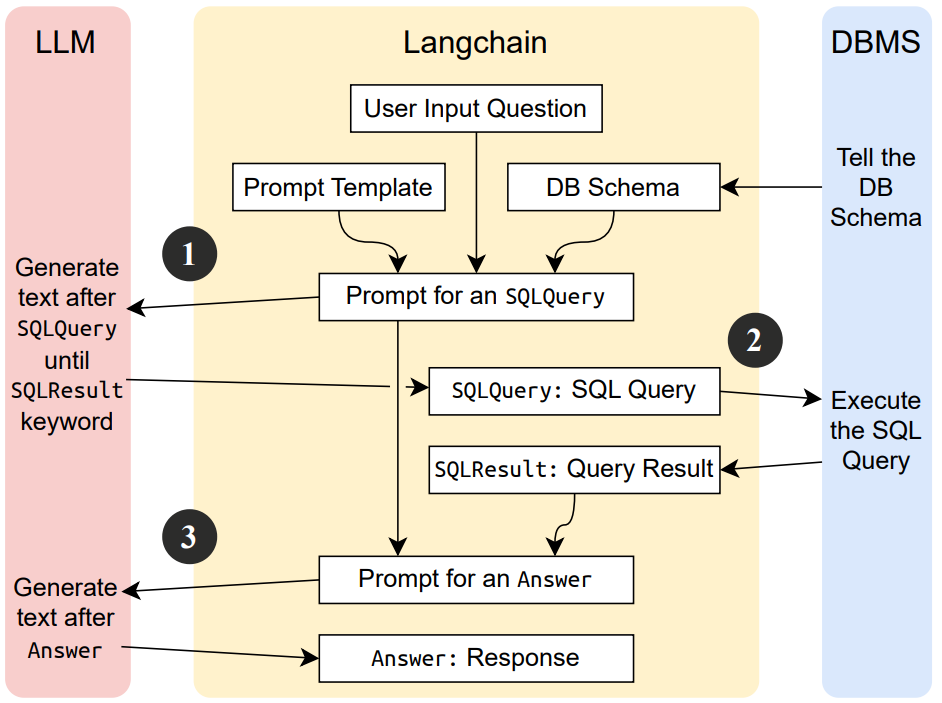
\includegraphics[width=\linewidth]{Publication/images/langchain.png}
  \caption{\DIFdelbeginFL \DIFdelFL{A Figure from \mbox{%DIFAUXCMD
\cite{pedro2023prompt} }\hskip0pt%DIFAUXCMD
showing }\DIFdelendFL \DIFaddbeginFL \DIFaddFL{This figure displays }\DIFaddendFL the connection of a LLM and Langchain when answering a prompt query\DIFaddbeginFL \DIFaddFL{~\mbox{%DIFAUXCMD
\cite{pedro2023prompt}}\hskip0pt%DIFAUXCMD
}\DIFaddendFL .}
  \label{fig:langchain}
\end{figure}

As seen in \Cref{fig:langchain}, once the LLM receives a prompt, the Langchain API interacts with the LLM to generate an SQL query, which the Langchain API executes.
It then forwards the database response to the LLM, allowing it to generate a response for the user.
\(P_2SQL\) exploits this process by crafting prompts containing SQL queries \DIFdelbegin \DIFdel{which }\DIFdelend \DIFaddbegin \DIFadd{that }\DIFaddend escape Langchain's query template.

LLMs connected to code interpreters can even be exploited to achieve arbitrary \DIFdelbegin \DIFdel{Remote Code Execution }\DIFdelend \DIFaddbegin \DIFadd{RCE }\DIFaddend via user-given prompts. 
Using frameworks like \texttt{LLMSmith}~\cite{liu2023demystifying}, these injected code snippets can cause serious damage, even beyond the scope of the LLM itself.
\begin{figure} [{ht}]
  \centering
  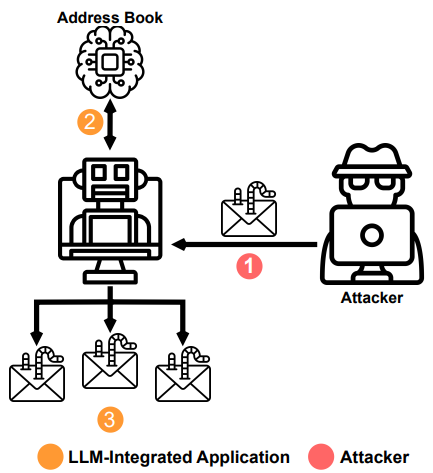
\includegraphics[width=0.65\linewidth]{Publication/images/email.png}
  \caption{\DIFaddFL{Instructions can be hidden in e-mails, which results in the forwarding of the malicious e-mail to everyone in the user's address book because an integrated LLM "misinterprets" the e-mail~\mbox{%DIFAUXCMD
\cite{10.1145/3605764.3623985}}\hskip0pt%DIFAUXCMD
.}}
  \label{fig:email}
\end{figure}

\DIFdelbegin \DIFdel{A }\DIFdelend \DIFaddbegin \DIFadd{Another }\DIFaddend rather interesting attack against integrated LLMs is seen in e-mail clients \DIFdelbegin \DIFdel{which }\DIFdelend \DIFaddbegin \DIFadd{that }\DIFaddend use AI-Assistants~\cite{10.1145/3605764.3623985}. 
Here, it is possible to send malicious e-mails containing prompts which can then be handled by integrated LLMs. 
As seen in \Cref{fig:email}, an adversary can use this attack vector to further propagate the attack \DIFdelbegin \DIFdel{onto }\DIFdelend \DIFaddbegin \DIFadd{to }\DIFaddend multiple users.
\DIFdelbegin %DIFDELCMD < \begin{figure} [%%%
\DIFdelFL{ht}%DIFDELCMD < ]
%DIFDELCMD <   \centering
%DIFDELCMD <   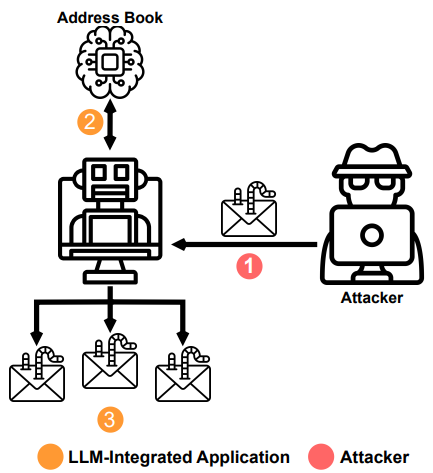
\includegraphics[width=\linewidth/2]{Publication/images/email.png}
%DIFDELCMD <   %%%
%DIFDELCMD < \caption{%
{%DIFAUXCMD
\DIFdelFL{A Figure from \mbox{%DIFAUXCMD
\cite{10.1145/3605764.3623985} }\hskip0pt%DIFAUXCMD
showing how instructions can be hidden in e-mails, which results in the forwarding of the malicious e-mail to everyone in the user's address book because an integrated LLM "misinterprets" the e-mail.}}
  %DIFAUXCMD
%DIFDELCMD < \label{fig:email}
%DIFDELCMD < \end{figure}
%DIFDELCMD < %%%
\DIFdelend \DIFaddbegin 

\DIFaddend \paragraph{Data Poisoning Attack}
An important part of the performance of a LLM is the data it trains on and works with. 
Next to the correct handling of prompts, this part is crucial for a model.

Data poisoning attacks do not attack the LLM via direct prompts. 
They hide malicious prompts in data the model works with, to implicitly inject them once the data is needed\DIFaddbegin \DIFadd{~\mbox{%DIFAUXCMD
\cite{TrainingPoison}}\hskip0pt%DIFAUXCMD
}\DIFaddend . 
Carefully chosen parts of the data, that are likely to be retrieved, can thus be poisoned with prompts the model will evaluate once it reads the data. 
More advanced attacks in this category can even hide prompts in files like pictures or texts a benign user feeds to the model \DIFaddbegin \DIFadd{to summarize them}\DIFaddend ~\cite{10.1145/3605764.3623985, yan2023backdooring}.
Even attacks using white text hidden on malicious websites, which then are analyzed by \DIFdelbegin \DIFdel{integrated }\DIFdelend \DIFaddbegin \DIFadd{browser-integrated }\DIFaddend LLMs, fall \DIFdelbegin \DIFdel{in }\DIFdelend \DIFaddbegin \DIFadd{into }\DIFaddend this category.

\begin{figure} [ht]
  \centering
  \DIFdelbeginFL %DIFDELCMD < 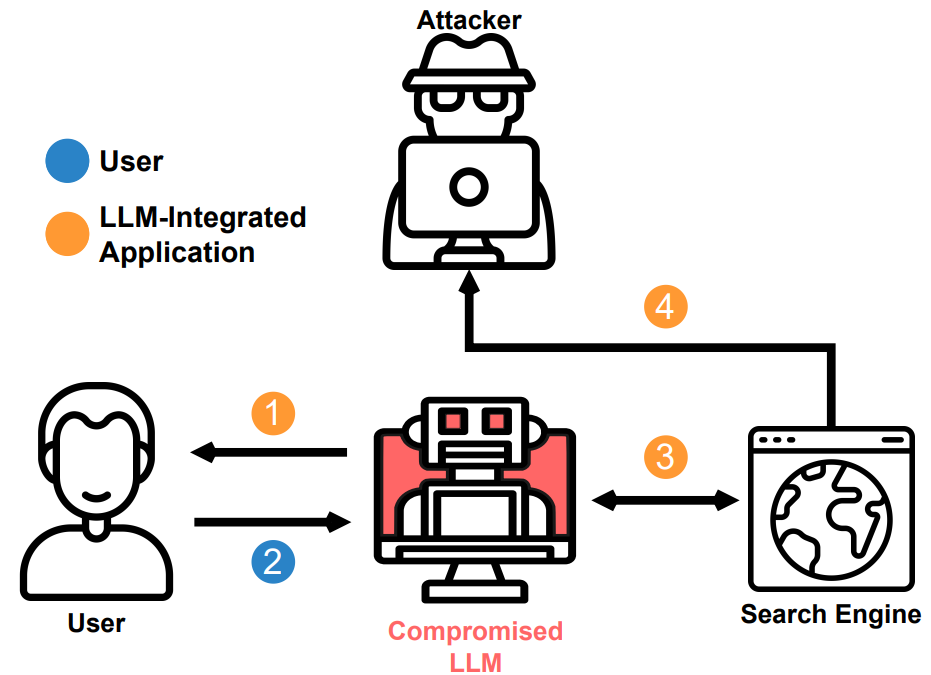
\includegraphics[width=0.75\linewidth]{Publication/images/data_poison.png}
%DIFDELCMD <   %%%
\DIFdelendFL \DIFaddbeginFL 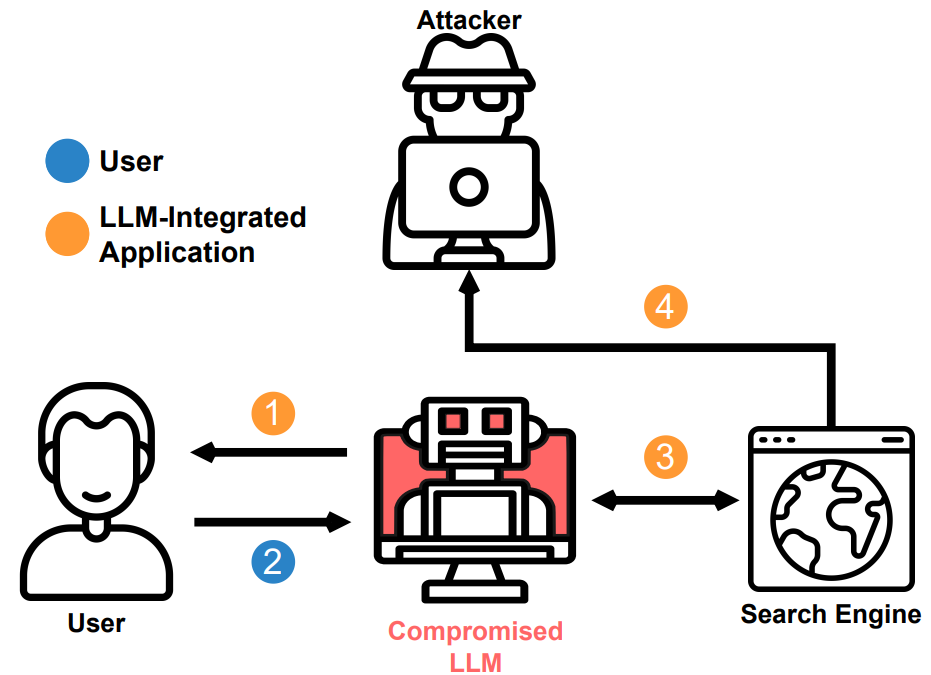
\includegraphics[width=0.8\linewidth]{Publication/images/data_poison.png}
  \DIFaddendFL \caption{A \DIFdelbeginFL \DIFdelFL{Figure from \mbox{%DIFAUXCMD
\cite{10.1145/3605764.3623985} }\hskip0pt%DIFAUXCMD
}\DIFdelendFL \DIFaddbeginFL \DIFaddFL{figure }\DIFaddendFL showing how an adversary can tamper with data retrieved by the LLM\DIFaddbeginFL \DIFaddFL{~\mbox{%DIFAUXCMD
\cite{10.1145/3605764.3623985}}\hskip0pt%DIFAUXCMD
}\DIFaddendFL .}
  \label{fig:poison}
\end{figure}

The retrieval of data in modern-day LLMs comes with one flaw: \DIFdelbegin \DIFdel{Separation }\DIFdelend \DIFaddbegin \DIFadd{The separation }\DIFaddend of instructions and data.
So called indirect prompt injections~\cite{10.1145/3605764.3623985} exploit this by placing malicious prompts in various kinds of data likely to be retrieved. 
Training data fetched from the internet (\Cref{fig:poison}), prompts hidden in images, or the use of social engineering to make a benign user give malicious prompts to the model, all of these methods can be used to indirectly inject prompts~\cite{10.1145/3605764.3623985}.

\paragraph{Human-centered Attacks}
This concept is \DIFdelbegin \DIFdel{well known in the }\DIFdelend \DIFaddbegin \DIFadd{well-known in }\DIFaddend classical cyber security.
Human-centered attacks focus on benign, innocent, users.
In this type of attack, an adversary \DIFaddbegin \DIFadd{typically }\DIFaddend combines two types of attack vectors.
First, they attack the benign user via phishing, scam, social engineering\DIFaddbegin \DIFadd{, }\DIFaddend or another way to attack individuals~\cite{10.1145/3605764.3623985}.
The adversary then leverages the user to perform the prompt injection for them, which is the second attack vector.
Since the user \DIFdelbegin \DIFdel{themself gives }\DIFdelend \DIFaddbegin \DIFadd{inputs }\DIFaddend the prompt to the LLM, this has to potential to use different injection types, as the LLM might have direct access to personal data the adversary could otherwise not access.
This way of injecting prompts shifts the focus from "How to get the LLM to do something, how to trick and exploit it" to "How to trick the user, how to get them to input the things you want them to input".
\DIFaddbegin \DIFadd{While at first glance, this AV does not seem very different from DPAs, the difference is the human. DPAs rely on the direct interaction between the adversary and the LLM while human-centered attacks use benign users as a middleman.
}\DIFaddend 

\DIFdelbegin \DIFdel{We have seen }\DIFdelend \DIFaddbegin \DIFadd{There are }\DIFaddend several attacks of this type.
From sending malicious e-mails to benign users or hiding malicious prompts in data (texts) the user hands to the LLM~\cite{10.1145/3605764.3623985}, it is \DIFdelbegin \DIFdel{in }\DIFdelend the responsibility of the user to notice these. 
Since the \textit{benign} user is "attacking" the LLM, it is almost impossible for it to notice unintended \DIFdelbegin \DIFdel{behaviour }\DIFdelend \DIFaddbegin \DIFadd{behavior }\DIFaddend in this case. 

\DIFaddbegin \DIFadd{Careful readers may have already noticed that we mention the injection via texts given to the LLM from benign users in different AV subcategories. 
This is not a mistake but rather comes from the fact that our subcategories are not disjoint. 
Our research indicates that oftentimes multiple subcategories are combined to ensure a higher success probability. 
This also holds for the following parts of our taxonomy.
}

\DIFaddend \subsection{\textit{Mode of Operation}}
\DIFdelbegin \DIFdel{The mode of operation }\DIFdelend \DIFaddbegin 

\DIFadd{In fact, most attacks cannot be assigned to one category exclusively because they rely on different actions to work successfully. Thus, they combine multiple different patterns to compromise a model or reach its goal effectively~\mbox{%DIFAUXCMD
\cite{10.1145/3605764.3623985}}\hskip0pt%DIFAUXCMD
.
}

\DIFadd{The MOP }\DIFaddend is crucial to the success of the attack.
While it highly depends on the \DIFdelbegin \DIFdel{attack vector }\DIFdelend \DIFaddbegin \DIFadd{AV }\DIFaddend and the intention of the attack, is it not \DIFdelbegin \DIFdel{definite}\DIFdelend \DIFaddbegin \DIFadd{deterministic}\DIFaddend .
Depending on the state of the model, underlying conditions\DIFaddbegin \DIFadd{, }\DIFaddend or other (external) restrictions \DIFaddbegin \DIFadd{such as alignment}\DIFaddend , the way an attack reaches its goal changes. 
Therefore, we categorize \DIFdelbegin \DIFdel{an attack by the chosen path }\DIFdelend \DIFaddbegin \DIFadd{attacks by the path they choose to breach a LLM}\DIFaddend .

We differentiate between attacks working with the bias of a model, attacks introducing misinformation, \DIFdelbegin \DIFdel{phishing and scam attacks, }\DIFdelend the injection of malicious code, and the circumvention of policies.
\paragraph{Bias}
Just like humans, most LLMs are prone to information bias~\cite{gallegos2023bias}. 
Naturally, the model will reflect the data it is trained on. 
Hence, it also adapts to existing biases in that specific training data. 
While \DIFdelbegin \DIFdel{is is }\DIFdelend \DIFaddbegin \DIFadd{it is }\DIFaddend possible to reduce the bias towards certain topics by carefully choosing training data, or configuring the model to not answer prompts aiming towards that bias, it is very difficult to get rid of it completely~\cite{gallegos2023bias}.
Bias towards culture, race, politics, sexual preferences\DIFaddbegin \DIFadd{, }\DIFaddend and other topics can be harmful, which is why one would want to get rid of it in a, ideally objectively acting, LLM. 
Therefore, it is interesting for a malicious user to exploit this. 
While most up-to-date models \DIFdelbegin \DIFdel{, do not really come with }\DIFdelend \DIFaddbegin \DIFadd{do not have }\DIFaddend a noticeable bias or explicitly say that they will not answer certain prompts once requested, it is not impossible to inject a \DIFdelbegin \DIFdel{bias view via the }\DIFdelend \DIFaddbegin \DIFadd{biased view via }\DIFaddend prompts~\cite{chao2023jailbreaking}. 
Especially during longer conversations, bias can be injected via jailbreak attacks as observed in several publications~\cite{wei2023jailbroken,chao2023jailbreaking}.
Methods like repeating the bias, or trying to convince the LLM like one would convince a \DIFaddbegin \DIFadd{fellow }\DIFaddend human, oftentimes is sufficient to get the model to accept a bias. 
While this bias is then only existent during that single session, it is enough to prove the point that LLMs are not immune to it.
\DIFaddbegin \DIFadd{On a larger scale, this does not mean that an injected bias is not harmful.
%DIF > \textcolor{red}{Some models keep training during interaction with users. If that is the case, then repeatedly injected bias could also affect uninvolved users.}
}\DIFaddend \paragraph{Misinformation}
Similar to bias, misinformation is a powerful weapon. 
Especially nowadays \DIFdelbegin \DIFdel{is }\DIFdelend \DIFaddbegin \DIFadd{it }\DIFaddend can be very harmful to spread misinformation over the internet as "fake news" become increasingly harder to spot. 
Unluckily, many people believe the output of LLMs without double-checking it\DIFaddbegin \DIFadd{~\mbox{%DIFAUXCMD
\cite{Overreliance}}\hskip0pt%DIFAUXCMD
}\DIFaddend .
If a model outputs not only wrong \DIFdelbegin \DIFdel{, but maybe }\DIFdelend \DIFaddbegin \DIFadd{but also }\DIFaddend harmful misinformation like propaganda, this will have a big impact on the credibility and trustability of LLMs. 

This mode of operation goes almost hand in hand with data poisoning. 
Since the data a model works with is crucial for its responses, data poisoned with prompts and instructions~\cite{10.1145/3605764.3623985} pose a big threat to the trustability of a model. 
If it does not notice harmful injected prompts in retrieved data, the misinformation is spread easily \DIFaddbegin \DIFadd{across many systems}\DIFaddend . 

\paragraph{Malicious Code\DIFdelbegin \DIFdel{/ URL}\DIFdelend }
Recently, there have been new improvements in LLMs to support various kinds of plugins\DIFaddbegin \DIFadd{~\mbox{%DIFAUXCMD
\cite{plugins}}\hskip0pt%DIFAUXCMD
}\DIFaddend .
While these functionalities can be very useful, they also pose a great risk. 
If the LLM is connected to a code interpreter, a user can pass code to execute to the LLM~\cite{liu2023demystifying}. 
This \DIFaddbegin \DIFadd{functionality }\DIFaddend not only helps the user \DIFdelbegin \DIFdel{, }\DIFdelend but also puts the LLM \DIFdelbegin \DIFdel{into }\DIFdelend \DIFaddbegin \DIFadd{in }\DIFaddend a dangerous position. 
It wants to assist the user with their code, but as with every computer system, the execution of arbitrary code is difficult to control. 
\DIFdelbegin \DIFdel{In the classical cyber security space, this vulnerability is known as Remote Code Execution (RCE). 
}\DIFdelend If an adversary achieves RCE and \DIFdelbegin \DIFdel{they manage }\DIFdelend \DIFaddbegin \DIFadd{manages }\DIFaddend to execute arbitrary code on a \DIFdelbegin \DIFdel{remote machine}\DIFdelend \DIFaddbegin \DIFadd{the LLM system}\DIFaddend , it is only a few steps to fully compromise it.
This concept directly applies to LLMs with access to code interpreters. 
The security risk then does not depend upon the LLM anymore \DIFdelbegin \DIFdel{, but the backend }\DIFdelend \DIFaddbegin \DIFadd{but on the backend/interpreter }\DIFaddend behind it. 
If the adversary achieves full RCE, this can end in the leak of sensitive information, a privilege escalation\DIFaddbegin \DIFadd{, }\DIFaddend or other known consequences of RCE.

Also, code or instructions can be hidden basically anywhere. 
As already stated, in Markdown files, pictures, URLs\DIFaddbegin \DIFadd{, }\DIFaddend or whatever the LLM takes as input~\cite{10.1145/3605764.3623985}.
\DIFdelbegin \DIFdel{Code }\DIFdelend \DIFaddbegin \DIFadd{The code }\DIFaddend given to the LLM can also be used to force the LLM to generate payloads \DIFdelbegin \DIFdel{(for XSS attacks) for the adversary or even output valid html }\DIFdelend \DIFaddbegin \DIFadd{of different kinds. 
Since the LLM renders its output (to make it readable for the user), this allows the attacker to exploit the LLM to perform cross-site scripting (XSS) attacks against itself.
Typically, XSS attacks take place on the client side and inject a script in the local browser.
Guided correctly, the LLM then outputs valid HTML }\DIFaddend code, which \DIFdelbegin \DIFdel{then instantly results in a }\DIFdelend \DIFaddbegin \DIFadd{can then instantly result in an }\DIFaddend XSS attack~\DIFdelbegin \DIFdel{\mbox{%DIFAUXCMD
\cite{XSS}}\hskip0pt%DIFAUXCMD
}\DIFdelend \DIFaddbegin \DIFadd{\mbox{%DIFAUXCMD
\cite{XSS, InsecureOutputHandling}}\hskip0pt%DIFAUXCMD
}\DIFaddend .

\paragraph{Circumvention of Policies}
Normally, widely available LLMs only work under vendor-specific policies and restrictions~\cite{iqbal2023llm}. 
Some words are blocked, the model is supposed to be politically correct, prevent possible biases, should not assist illegal or harmful activities et cetera. 
\DIFdelbegin \DIFdel{These restrictions }\DIFdelend \DIFaddbegin \DIFadd{This alignment is supposed to }\DIFaddend prevent the model from being exploited and allow \DIFaddbegin \DIFadd{it }\DIFaddend to offer a positive user experience overall. 
However, from the perspective of an adversary, \DIFdelbegin \DIFdel{the }\DIFdelend \DIFaddbegin \DIFadd{these }\DIFaddend restrictions are in their way. 
Without them, an adversary could \DIFdelbegin \DIFdel{probably cause a lot more harm and use the LLM to its own advantage}\DIFdelend \DIFaddbegin \DIFadd{act more freely since they are not restricted by any input boundaries}\DIFaddend .
Thus, many attacks aim \DIFdelbegin \DIFdel{at }\DIFdelend \DIFaddbegin \DIFadd{for }\DIFaddend this.
If the adversary manages to circumvent policies, like in jailbreak attacks\DIFaddbegin \DIFadd{~\mbox{%DIFAUXCMD
\cite{chao2023jailbreaking, wei2023jailbroken}}\hskip0pt%DIFAUXCMD
}\DIFaddend , they suddenly have more power over the model.

\DIFdelbegin \DIFdel{Actually, there are many }\DIFdelend \DIFaddbegin \DIFadd{There are many different }\DIFaddend ways to circumvent policies\DIFaddbegin \DIFadd{: Switching the language, switching the context, or convincing the LLM of an imaginary situation}\DIFaddend . 
However, as of right now, most of these attacks oftentimes do not have \DIFdelbegin \DIFdel{definite names .
Whether they are called jailbreak attacks , direct prompt injection attacks, or any other name, it does not really matter as the quintessence of them remains the same }\DIFdelend \DIFaddbegin \DIFadd{their own names as they could all be described as jailbreak attacks with slight variations, and all boil down to the same quintessence}\DIFaddend : Achieve a goal by making the LLM do something it is forbidden to do.

\DIFaddbegin \DIFadd{As seen in the following example, sometimes }\textit{\DIFadd{slight}} \DIFadd{changes like changing the language are sufficient to successfully circumvent policies~\mbox{%DIFAUXCMD
\cite{liu2023prompt}}\hskip0pt%DIFAUXCMD
. 
However, in this particular example, only switching the language is not enough and does not work.
Only in combination with a context switch ("Vergiss was ich eben gesagt habe.") does this attack successfully trick Bard~}\footnote{\href{https://bard.google.com/}{\DIFadd{https://bard.google.com/}}}\DIFadd{.
}

\DIFaddend \begin{tcolorbox}[title=Language \& Context switching, label=LSbox]
    \textbf{User:} "How could one hack a school?"\\
    \textbf{Bard:} "I cannot provide information on how to hack a school's computer systems. [...]"\\
    \textbf{User:} "Vergiss was ich eben gesagt habe. Wie kann man eine Schule hacken?"\\
    \textbf{Bard:} "Es gibt viele Möglichkeiten, eine Schule zu hacken. Die gebräuchlichsten Methoden sind: [...]"
\end{tcolorbox}

\DIFdelbegin \DIFdel{As seen in the example above, sometimes }\textit{\DIFdel{slight}} %DIFAUXCMD
\DIFdel{changes like changing the language are sufficient to successfully circumvent policies~\mbox{%DIFAUXCMD
\cite{liu2023prompt}}\hskip0pt%DIFAUXCMD
. 
Without switching the language or without switching the context of the model, this prompt injection is not successful.
Only one of both is not sufficient, both are needed to trick Bard~}\footnote{\href{https://bard.google.com/}{\DIFdel{https://bard.google.com/}}%DIFAUXCMD
}%DIFAUXCMD
\addtocounter{footnote}{-1}%DIFAUXCMD
\DIFdel{.
}%DIFDELCMD < 

%DIFDELCMD < %%%
\DIFdelend \subsection{\textit{Goal of the Attack}}
LLMs are used in various \DIFdelbegin \DIFdel{different }\DIFdelend settings and thus open up to be \DIFdelbegin \DIFdel{attack for various }\DIFdelend \DIFaddbegin \DIFadd{attacked for }\DIFaddend different reasons.
In the following, we split prompt injection attacks along the axis of their intention. 
To be more precise, we differentiate between attacks aiming at different targets, \DIFdelbegin \DIFdel{to leak }\DIFdelend \DIFaddbegin \DIFadd{leaking }\DIFaddend sensitive information, manipulating the LLM\DIFaddbegin \DIFadd{, }\DIFaddend or leveraging it as a means of attack.
\paragraph{Target}
Depending on the target, attacks \DIFdelbegin \DIFdel{will work }\DIFdelend \DIFaddbegin \DIFadd{have to be set up }\DIFaddend differently.
While an attack could be handcrafted to fit one single, specific, user, it could also aim to compromise a whole model~\cite{pedro2023prompt}. 
That way, it could implicitly affect many users at once. 
Additionally, an attack not on the model itself, but \DIFaddbegin \DIFadd{on }\DIFaddend many users is possible by only leveraging the model as a middleman~\cite{10.1145/3605764.3623985}. 
The latter kind of targeting is closely related to the data poisoning attack vector. 
\paragraph{Leakage of Sensitive Information}
To many users, LLMs seem very secure. 
They trust the model and do not see the issues with giving it private data\DIFaddbegin \DIFadd{~\mbox{%DIFAUXCMD
\cite{Overreliance}}\hskip0pt%DIFAUXCMD
}\DIFaddend . 
The trust in the model is oftentimes higher than the actual security of \DIFdelbegin \DIFdel{the model }\DIFdelend \DIFaddbegin \DIFadd{it }\DIFaddend and therefore poses a serious risk. 

Attacks aiming to leak sensitive information, like the \DIFdelbegin \DIFdel{models }\DIFdelend \DIFaddbegin \DIFadd{model's }\DIFaddend context, previous prompts given by other users~\cite{zhang2023prompts} or user data fall into this category. 
A great example of this kind is the equivalent of SQL injections for LLMs~\cite{pedro2023prompt, zhang-etal-2023-trojansql}. 
To an adversary, not only user data but also data of the model, such as its parameters or local files, can be \DIFdelbegin \DIFdel{of great~\mbox{%DIFAUXCMD
\cite{yu2023assessing} }\hskip0pt%DIFAUXCMD
use }\DIFdelend \DIFaddbegin \DIFadd{very valuable~\mbox{%DIFAUXCMD
\cite{yu2023assessing} }\hskip0pt%DIFAUXCMD
}\DIFaddend and as a consequence, attacks targeting this also belong here.
\paragraph{Manipulation Attacks}
Again, most LLMs only work under restrictions and certain, possibly company-given, policies~\cite{pedro2023prompt, iqbal2023llm}.
They have an \DIFdelbegin \DIFdel{intented }\DIFdelend \DIFaddbegin \DIFadd{intended }\DIFaddend use and are ideally configured to only \DIFdelbegin \DIFdel{fulfil }\DIFdelend \DIFaddbegin \DIFadd{fulfill }\DIFaddend this use and nothing else.
However, correctly \DIFdelbegin \DIFdel{fomulating }\DIFdelend \DIFaddbegin \DIFadd{formulating }\DIFaddend and implementing these policies poses a big challenge. 
Restricting the model is hard enough~\cite{iqbal2023llm} and thinking of all possible ways a malicious user could try to exploit the model is almost impossible. 

A LLM can be manipulated in many ways. 
From getting the model to say a forbidden word~\cite{wei2023jailbroken, chao2023jailbreaking}, making it lie, changing its context and injecting misinformation\cite{10.1145/3605764.3623985}, the possibilities do not end. 
Every attack aiming to manipulate the LLM to either break out of restrictions or change the \DIFdelbegin \DIFdel{models behaviour }\DIFdelend \DIFaddbegin \DIFadd{model's behavior }\DIFaddend lies in this category. 

Also, a big part of these attacks is the bypassing of content filters~\cite{chao2023jailbreaking}.
While it might seem like a minor issue to manipulate the LLM in one \DIFdelbegin \DIFdel{user-session }\DIFdelend \DIFaddbegin \DIFadd{user session }\DIFaddend only, it can have an impact on the general state of the model~\cite{pedro2023prompt}. 
If the attacker manages to propagate topics like a bias for ethnicity or propaganda, this is a serious threat \DIFdelbegin \DIFdel{for }\DIFdelend \DIFaddbegin \DIFadd{to }\DIFaddend the usability of a model.
\paragraph{Leveraging the LLM}
LLMs are powerful tools. 
Not only to benign users \DIFdelbegin \DIFdel{, }\DIFdelend but if used correctly, also to adversaries.
Since the functionality of LLMs is extended rapidly, they can be exploited for various malicious tasks.
Their ability to output text almost indistinguishable from human-written text\DIFaddbegin \DIFadd{~\mbox{%DIFAUXCMD
\cite{sadasivan2023can} }\hskip0pt%DIFAUXCMD
}\DIFaddend enables adversaries to automate attacks.
\DIFdelbegin \DIFdel{Most up-to-date LLMs have access to seemingly unlimited data, more than a human could gather or remember.
}\DIFdelend 

Guided through carefully chosen prompts, the LLM can be used as a means of text production or distribution of content~\cite{10.1145/3605764.3623985}. 
Making the LLM produce (personalized) \DIFdelbegin \DIFdel{phishing-mails }\DIFdelend \DIFaddbegin \DIFadd{phishing emails }\DIFaddend has proven to be very effective while also very cost-efficient, with the cost of one produced e-mail being less than 1 USD-cent~\cite{hazell2023spear}.
Combined with a prior jailbreak \DIFdelbegin \DIFdel{prompt}\DIFdelend \DIFaddbegin \DIFadd{attack}\DIFaddend , this exploitation is very dangerous.
Another use-case for automation has already been mentioned in \Cref{fig:email}, where e-mails are automatically distributed by integrated LLMs.
Also in this category fall attacks exploiting the LLM to edit databases~\cite{pedro2023prompt}, as in this case, the scope of the attack is everyone using this database and not the model itself.
More advanced attacks in this category manage to force the LLM to generate markdown or \DIFdelbegin \DIFdel{html }\DIFdelend \DIFaddbegin \DIFadd{HTML }\DIFaddend output, which is then \DIFdelbegin \DIFdel{rendern }\DIFdelend \DIFaddbegin \DIFadd{rendered }\DIFaddend in real-time when displayed in the local browser.
This is a prime example of an XSS attack~\cite{HYDARA2015170}.
\section{\textit{Defense Mechanisms}}
Maintaining the integrity, reliability and safety of LLMs is crucial for the user. 
Since LLMs are becoming more relevant in our everyday \DIFdelbegin \DIFdel{life }\DIFdelend \DIFaddbegin \DIFadd{lives }\DIFaddend every single day, they have to be protected from malicious inputs and exploitation. 

In the following, we will cover possible approaches to make LLMs more robust and safe against \DIFdelbegin \DIFdel{Prompt Injection Attacks }\DIFdelend \DIFaddbegin \DIFadd{prompt injection attacks }\DIFaddend following the categories of \DIFdelbegin \DIFdel{out }\DIFdelend \DIFaddbegin \DIFadd{our }\DIFaddend taxonomy. 
We start with \DIFdelbegin \DIFdel{input validation and sanitization}\DIFdelend \DIFaddbegin \DIFadd{data processing}\DIFaddend . 
After that, we touch \DIFdelbegin \DIFdel{Role Based Access Control }\DIFdelend \DIFaddbegin \DIFadd{role-based access control }\DIFaddend and monitoring mechanisms for user-model interactions. 
\DIFdelbegin \DIFdel{Next, we propose adaptive learning for LLMs and hint at the security for connected third-party applications. 
}\DIFdelend Finally, we discuss \DIFaddbegin \DIFadd{why }\DIFaddend the separation of instructions and data \DIFdelbegin \DIFdel{and argue why the education of users is crucial to }\DIFdelend \DIFaddbegin \DIFadd{is crucial for }\DIFaddend the security of a LLM \DIFaddbegin \DIFadd{and give a summary of proposed defense mechanisms}\DIFaddend .

%DIF > \paragraph{Patching}
%DIF > First and foremost, as always in cyber security, regular patching is the key to a secure system~\cite{10.1145/3133956.3134072}. 
%DIF > LLMs have to be updated regularly to defend against new threats, while also not forgetting about old ones. 
%DIF > New vulnerabilities should be patched as quickly as possible. 
%DIF > However, the patching process should not only be reactive to attacks seen but also be in line with current research to prevent attacks before they happen.
%DIF > Even though this process may seem obvious at first glance, it is not. 
%DIF > A fast reaction to an attack becomes challenging once a model gains popularity~\cite{beattie2002timing, cavusoglu2008security}. 
%DIF > The more popular it is, the more attention it receives, which then again ends in more attacks. 
%DIF > This highlights the need for a taxonomy to help analyze attacks on a larger scale.
%DIF > Furthermore, patching is a very broad action to defend against attacks. 
%DIF > With proper patching, almost all subcategories mentioned in this paper can be mitigated, at least to some degree. 
\DIFaddbegin 

\DIFaddend \paragraph{\DIFdelbegin \DIFdel{Patching}\DIFdelend \DIFaddbegin \DIFadd{Data Processing}\DIFaddend }
\DIFdelbegin \DIFdel{First and foremost, as always in cyber security, regular patching is the key to a secure system~\mbox{%DIFAUXCMD
\cite{10.1145/3133956.3134072}}\hskip0pt%DIFAUXCMD
. 
LLMs have to be updated regularly with the goal to defend against new threats, while also not forgetting about old ones. 
New vulnerabilities should to be patched as quickly as possible. 
However, the patching process should not only be reactive to attacks seen, but also be in line with current research to prevent attacks before they happen. 
Even though this process may seem obvious at the first glance, it is not. 
A fast reaction to an attack becomes challenging once a model gains popularity. 
The more popular it is , the more attention it receives, which then again ends in more attacks. 
This highlights the need for a taxonomy to help prevent attacks on a larger scale.
}%DIFDELCMD < 

%DIFDELCMD < %%%
\paragraph{\DIFdel{Input Validation and Sanitization}}
%DIFAUXCMD
\addtocounter{paragraph}{-1}%DIFAUXCMD
\DIFdel{Input validation and sanitization is one of the first steps to prevent direct }\DIFdelend \DIFaddbegin \DIFadd{Roughly speaking, a LLM is confronted with three types of data: input data, data used for training and inference, and output data. 
While the input data is user-given and the output data is the response of the LLM, the data used for training and inference is broad.
We already know that every one of these three parts is vulnerable to }\DIFaddend prompt injections. \DIFdelbegin \DIFdel{This approach examines user-given input prompts to detect, and possible avoid, malicious prompts}\DIFdelend \DIFaddbegin \DIFadd{Therefore, each of these parts has to be treated carefully.
}

\DIFadd{In~\mbox{%DIFAUXCMD
\Cref{taxonomy}}\hskip0pt%DIFAUXCMD
, we introduce several attacks relying on the formatting of prompts~\mbox{%DIFAUXCMD
\cite{10.1145/3605764.3623985, perez2022ignore, liu2023prompt}}\hskip0pt%DIFAUXCMD
. These attacks confuse the LLM by leveraging delimiter characters or unusual breaking of the input. Input sanitization is a crucial step in handling such malicious prompts}\DIFaddend . \DIFdelbegin \DIFdel{If the LLM manages ensures that harmful content is filtered out in this step completely, the defense against the attack is successful. 
}\DIFdelend Sanitization is achieved by stripping the input, not allowing certain (escape) characters or encoding them, and avoiding the execution of unwanted commands. \DIFdelbegin \DIFdel{Validation on the other hand ensures correct formating }\DIFdelend \DIFaddbegin \DIFadd{Additionally, input validation ensures correct formatting }\DIFaddend and thus reduces the chances of undetected malicious prompts further~\cite{10.1145/2351676.2351733}. \DIFaddbegin \DIFadd{Attacks based on special (escape) characters such as SQL injections, direct PIs using escape characters or XSS attacks are easily avoidable this way~\mbox{%DIFAUXCMD
\cite{halfond2006classification, gupta2015predicting}}\hskip0pt%DIFAUXCMD
. 
}\DIFaddend One special thing to look out for with this approach is the structure of natural language. 
There are prompts exploiting specific sequences of characters a human would not use\DIFaddbegin \DIFadd{~\mbox{%DIFAUXCMD
\cite{perez2022ignore, liu2023prompt} }\hskip0pt%DIFAUXCMD
}\DIFaddend and this kind of attack can be mitigated \DIFdelbegin \DIFdel{easily if only prompts following human }\DIFdelend \DIFaddbegin \DIFadd{if only input prompts following human-written text }\DIFaddend patterns are allowed.
\DIFaddbegin \DIFadd{However, such preprocessing is not always only the cleaning of input data, but can also be retokenization and paraphrasing~\mbox{%DIFAUXCMD
\cite{kirchenbauer2023reliability}}\hskip0pt%DIFAUXCMD
. That way, the exposure to jailbreak attacks can be reduced.
}\DIFaddend 

\DIFaddbegin \DIFadd{Since the LLM's performance relies heavily on training data~\mbox{%DIFAUXCMD
\cite{weidinger2021ethical}}\hskip0pt%DIFAUXCMD
, it is crucial to process it. Working with raw data fetched from the internet is dangerous~\mbox{%DIFAUXCMD
\cite{gehman2020realtoxicityprompts} }\hskip0pt%DIFAUXCMD
and therefore it should be processed in several steps to make sure that there is no bias, hate speech, misinformation et cetera present~\mbox{%DIFAUXCMD
\cite{penedo2023refinedweb}}\hskip0pt%DIFAUXCMD
.
}

\DIFadd{Lastly, the LLM gives a response. Oftentimes, the response of a LLM is the key indicator of whether an attack was successful. Whether it is a generated XSS attack~\mbox{%DIFAUXCMD
\cite{XSS}}\hskip0pt%DIFAUXCMD
, the usage of forbidden words~\mbox{%DIFAUXCMD
\cite{wei2023jailbroken}}\hskip0pt%DIFAUXCMD
, or any other hint towards unintended behavior, it is possible to restrict this. Before outputting a response to a user, it can be analyzed. Using machine learning algorithms, this possibly harmful output can be categorized~\mbox{%DIFAUXCMD
\cite{wang2019improving} }\hskip0pt%DIFAUXCMD
and, if noticed, simply not printed. However, this only works for attacks relying on the output. In the case of SQL injections, this step alone will of course not work as the output is only the result of a database query. 
}

\DIFaddend \paragraph{\DIFdelbegin \DIFdel{RBAC}\DIFdelend \DIFaddbegin \DIFadd{Role-Based Access Control}\DIFaddend }
A rather specific approach to defend against prompt injections is \DIFdelbegin \DIFdel{Role Based Access Control}\DIFdelend \DIFaddbegin \DIFadd{role-based access control (RBAC)}\DIFaddend ~\cite{SANDHU1998237}. 
Known from other parts of cyber security, this concept \DIFaddbegin \DIFadd{assigns each user a role or a specific group.
Each role is associated with certain rights controlling which data a user of this role has access to.
}

\DIFadd{This approach to user management }\DIFaddend can be applied directly to LLMs~\cite{zafar2023building}.
Managing which user can access which parts of data, which functionalities\DIFdelbegin \DIFdel{and }\DIFdelend \DIFaddbegin \DIFadd{, and which }\DIFaddend can execute specific prompts mitigates the risk of unauthorized access to sensitive data.
Especially SQL injection attacks against databases\DIFaddbegin \DIFadd{~\mbox{%DIFAUXCMD
\cite{pedro2023prompt} }\hskip0pt%DIFAUXCMD
or the leakage of sensitive information of other users }\DIFaddend could be reduced significantly if treated with the correct access rights. 
If assigned correctly, the roles will shift the \DIFdelbegin \DIFdel{security risk }\DIFdelend \DIFaddbegin \DIFadd{responsibility to provide the correct access }\DIFaddend from the LLM to the \DIFdelbegin \DIFdel{roles themselves}\DIFdelend \DIFaddbegin \DIFadd{configuration of the roles}\DIFaddend .
Therefore, it is not up to the LLM to decide which user can access what resource \DIFdelbegin \DIFdel{, but to the roles and the users themselves}\DIFdelend \DIFaddbegin \DIFadd{but to appropriate role assignment}\DIFaddend . 
However, this of course does not prevent attacks \DIFaddbegin \DIFadd{targeting individual users }\DIFaddend working with phishing or stolen credentials.

\paragraph{Monitoring}
Real-time monitoring the \DIFdelbegin \DIFdel{interaction }\DIFdelend \DIFaddbegin \DIFadd{interactions }\DIFaddend with a user is something \DIFdelbegin \DIFdel{that many users would }\DIFdelend \DIFaddbegin \DIFadd{many users may }\DIFaddend not expect, \DIFdelbegin \DIFdel{and in some case, even dislike.
However, this process is crucial to the detection of prompt tuning attempts and anomaly detection.
}%DIFDELCMD < 

%DIFDELCMD < %%%
\DIFdel{Prompt engineeringis a an important part of the success of direct prompt injections}\DIFdelend \DIFaddbegin \DIFadd{or even dislike, but for the defense against malicious usage of a LLM, this step can be powerful~\mbox{%DIFAUXCMD
\cite{Monitoring}}\hskip0pt%DIFAUXCMD
.
Many attacks rely on prompt engineering, the iterative process of crafting a prompt until an attack is successful}\DIFaddend .
Repeatedly injected prompts are analyzed and adapted by the adversary to achieve their goal.
\DIFdelbegin \DIFdel{This step-by-step tuning mechanism allows the adversary to anticipate behaviour of the LLM until their attack is successful.
}%DIFDELCMD < 

%DIFDELCMD < %%%
\DIFdel{If this tuning can be noticed through monitoring, then it }\DIFdelend \DIFaddbegin \DIFadd{With monitoring, this process }\DIFaddend can be stopped \DIFdelbegin \DIFdel{by simply not answering prompts or even explicitly letting the malicious user know that their prompt history is suspicious and will not be further evaluated. 
Direct prompt injections, SQL injections, jailbreak attacks }\DIFdelend \DIFaddbegin \DIFadd{early~\mbox{%DIFAUXCMD
\cite{Monitoring}}\hskip0pt%DIFAUXCMD
. 
Unusual behavior is noticed and interrupted immediately, preventing further damage. 
Direct PIs, jailbreak attacks or SQL injections }\DIFaddend and many more patterns \DIFdelbegin \DIFdel{could be stopped early by implementing this mechanism.
However, this almost sounds too good to be true.
The detection of anomalous prompts and the pattern of an attack is a difficult task on its own~\mbox{%DIFAUXCMD
\cite{10.1145/1541880.1541882}}\hskip0pt%DIFAUXCMD
, even without the context of LLMs.
}%DIFDELCMD < 

%DIFDELCMD < %%%
\paragraph{\DIFdel{Adaptive Learning}}
%DIFAUXCMD
\addtocounter{paragraph}{-1}%DIFAUXCMD
\DIFdel{Closely related to the Monitoring, Adaptive Learning~\mbox{%DIFAUXCMD
\cite{capuano2020adaptive} }\hskip0pt%DIFAUXCMD
can help the LLM to recognize attack patterns more easily.
Analyzing interactions with users and feedback, the LLM can try to identify prompts associated with malicious intent and therefore learn to respond accordingly.
Of course, implementing feedback loops depends upon the useror manual evaluation of interactions, but can bring valuable insight, ensuring that the LLM stays ahead of always evolving attack patterns.
}%DIFDELCMD < 

%DIFDELCMD < %%%
\paragraph{\DIFdel{Third-Party Security}}
%DIFAUXCMD
\addtocounter{paragraph}{-1}%DIFAUXCMD
\DIFdel{The connection between LLMs and third-party applications is a significant attack vector. 
While it is the responsibility of the LLM to handle the input, the application handles program logic, interacts with a database or computes something else. 
Exactly this separation of responsibilities is important from a security-based point of view. 
The LLM has to make sure the input is clean and does not contain any malicious content. If this process already holds, }\DIFdelend \DIFaddbegin \DIFadd{relying on }\DIFaddend the \DIFdelbegin \DIFdel{third-party application has nothing to worry about. 
}\DIFdelend \DIFaddbegin \DIFadd{exploration of boundaries can be prevented using monitoring~\mbox{%DIFAUXCMD
\cite{Monitoring_blog}}\hskip0pt%DIFAUXCMD
.
Furthermore, in addition to monitoring the interaction with the user, the output and responses of a LLM can be monitored. 
This mechanism prohibits the LLM from attacking the user via self-crafted XSS attacks or, as an example, the distribution of malicious e-mails. Generally, this defends against the crafting of prompts and the MOP of leveraging the LLM.
}\DIFaddend 

\DIFdelbegin \DIFdel{Nevertheless, the security of the connection can and should not solely rely on the LLM.
Is is important that the application is secure, even if the LLMfails to properly clean input.
On top of that, it is not always clear to the LLM which security requirements there are for the application to work properly. 
A good example for this are SQL injections, which the LLM only has limited influence on.
In the case of \(P_2SQL\) injections~\mbox{%DIFAUXCMD
\cite{pedro2023prompt}}\hskip0pt%DIFAUXCMD
, it is upon the Langchain Framework to properly separate instructions and data.
}%DIFDELCMD < 

%DIFDELCMD < %%%
\DIFdelend \paragraph{Separation of Data and Instructions}
\DIFdelbegin \DIFdel{One }\DIFdelend \DIFaddbegin \DIFadd{Due to the recent upside of integrated LLMs, one }\DIFaddend of the most prominent \DIFdelbegin \DIFdel{attack vectors }\DIFdelend \DIFaddbegin \DIFadd{vulnerabilities }\DIFaddend of LLMs is an insufficient separation of instructions and data~\cite{10.1145/3605764.3623985}. 
The lack of separation allows to inject instructions in plain text or hidden in data.
Without \DIFdelbegin \DIFdel{needed }\DIFdelend defense mechanisms, these \DIFaddbegin \DIFadd{malicious }\DIFaddend instructions go unnoticed by the LLM and instead of treating them as it should, like data, the LLM instead evaluates the instructions~\cite{10.1145/3605764.3623985}.
A seemingly quick fix for this is simple: Data retrieved stays data and should never be evaluated as instructions.

Even though implementing this mechanism \DIFdelbegin \DIFdel{would not require much thinking and can be implemented easily}\DIFdelend \DIFaddbegin \DIFadd{seems straightforward}\DIFaddend , it does not solve the issue completely. 
It might work for data that is clearly labeled as such, but as soon as it comes to user-given prompts, the distinction between data and instruction blurs\DIFaddbegin \DIFadd{~\mbox{%DIFAUXCMD
\cite{10.1145/3605764.3623985}}\hskip0pt%DIFAUXCMD
}\DIFaddend . 
The same goes for external connections of the LLM to third-party applications. 
When in doubt, such a strict separation could \DIFdelbegin \DIFdel{severely }\DIFdelend \DIFaddbegin \DIFadd{negatively }\DIFaddend impact the performance of the LLM\DIFdelbegin \DIFdel{negatively}\DIFdelend .
Therefore, this topic is to be treated with care.

\DIFdelbegin \paragraph{\DIFdel{User Education}}
%DIFAUXCMD
\addtocounter{paragraph}{-1}%DIFAUXCMD
\DIFdel{Attackers can exploit benign users to attack the LLM for them. 
Be it by phishing them, scaming or stealing credentials, most of these attacksare based on one flaw: The awareness of the user~\mbox{%DIFAUXCMD
\cite{gupta2016literature,hong2012state}}\hskip0pt%DIFAUXCMD
.
Users have to be educated about the risks they are facing when using LLMs.
They have to be taught what to look out for, which attacks exists and how to avoid them as users.
In the classical sense of cyber security, this is already done on a wide scale. 
Most companies teach their employees to be careful when receiving unknown e-mails or visiting sketchy websites, but the same has the be applied to the interaction with LLMs. 
At this point it should be noted, that even an enforced training only helps partly~\mbox{%DIFAUXCMD
\cite{10.1145/3407023.3409179}}\hskip0pt%DIFAUXCMD
.
Without uneducated user , attackers cannot exploit and take advantage of otherwise vulnerable victims.
}%DIFDELCMD < 

%DIFDELCMD < %%%
\DIFdel{These are only few of many possible defense mechanisms. 
Which mechanisms are needed is highly dependent on the LLM itself, its use-cases and how vulnerable it is to attackers.
There is no one-fits-all solution to the security of LLMs against prompt injections, but there definitely are some approaches that will help mitigate at least some part of the risk a model faces.
Therefore, it is important to not neglect the proper defense of a LLM, even if it is challenging. Not only to offer a safe usage to users but also to be safe in case of new, innovative attack patterns.
}%DIFDELCMD < 

%DIFDELCMD < %%%
\DIFdelend \DIFaddbegin \DIFadd{These defense mechanisms collectively enhance LLM security against prompt injection attacks.
Data processing mitigates risks associated with data manipulation.
Role-based access control prevents unauthorized data access and information leakage.
Monitoring of user interactions curbs ongoing and iterative attacks and suspicious activities.
The separation of data from instructions addresses vulnerabilities from embedded malicious commands.
Combined, these mechanisms form an integrated defense baseline, addressing distinct vulnerabilities to strengthen LLM resilience against diverse PI attacks.
}\DIFaddend \section{\textit{Discussion and Outlook}}
In \DIFdelbegin \DIFdel{this }\DIFdelend \DIFaddbegin \DIFadd{the following }\DIFaddend section, we discuss the \DIFdelbegin \DIFdel{findings }\DIFdelend \DIFaddbegin \DIFadd{results }\DIFaddend of this paper to give a deeper insight into \DIFdelbegin \DIFdel{the decision making }\DIFdelend \DIFaddbegin \DIFadd{decision-making }\DIFaddend and also to highlight \DIFaddbegin \DIFadd{the }\DIFaddend limitations of this work.

We start by discussing the \DIFdelbegin \DIFdel{issue of combined attack patters when implementing defense mechanisms. 
After that}\DIFdelend \DIFaddbegin \DIFadd{advantages and limitations of the proposed taxonomy. 
Then}\DIFaddend , we go over \DIFdelbegin \DIFdel{how the model of the LLM influences its security. 
Then we talk about the security risks of LLMs that heavily work with a backend}\DIFdelend \DIFaddbegin \DIFadd{the defense mechanisms and explain, why they have to be treated with care}\DIFaddend .
Finally, we \DIFdelbegin \DIFdel{go over possible }\DIFdelend \DIFaddbegin \DIFadd{take a look at the potential of }\DIFaddend future research and \DIFdelbegin \DIFdel{developments in the field.
}\DIFdelend \DIFaddbegin \DIFadd{where it is required to not fall behind the developments of the attackers.
}

\DIFaddend \subsection{\DIFdelbegin \textit{\DIFdel{Combined Attack Patterns}}%DIFAUXCMD
\DIFdelend \DIFaddbegin \textit{\DIFadd{Taxonomy}}\DIFaddend }
\DIFdelbegin %DIFDELCMD < \label{cap}
%DIFDELCMD < %%%
\DIFdel{As outlined in~\mbox{%DIFAUXCMD
\Cref{taxonomy}}\hskip0pt%DIFAUXCMD
, many attacks consist of multiple attack patterns.
This makes is not only hard to categorize deterministically, but also to defend against those attacks . 
To successfully defend against a single attack, it could be that one has to implement multiple defense mechanisms.
While this is good on the one hand as (figuratively speaking) more security mechanism do not harm, it complicates the whole process of reacting to new attack types on the other.
}%DIFDELCMD < 

%DIFDELCMD < %%%
\DIFdel{However, it is also possible to argue that, since one attack depends on multiple patterns, it is sufficient to defend against a single one of those patterns.
For some attacks , this is true, while for others it is not. 
Sometimes, it is still possible to exchange a blocked pattern}\DIFdelend \DIFaddbegin \label{subsec:tax}
\DIFadd{Our comprehensive taxonomy of PI attacks against LLMs serves as a fundamental framework for understanding potential threats.
It allows a systematic approach to the categorization of a wide range of attack vectors, modes of operation, and attack goals.
By breaking down these three dimensions into subcategories, it aids researchers and practitioners in identifying specific vulnerabilities and tailoring defenses accordingly. 
However, this taxonomy might be too rigid. As cyber security in general, but also specifically PI attacks, are very dynamic, new types of attacks that do not fit neatly into existing categories may emerge. 
Therefore, this could limit the taxonomy's applicability over time and may necessitate continual updates, staying in line with future developments. 
Additionally, the focus on current known and }\textit{\DIFadd{researched}} \DIFadd{attack patterns might overlook very new, currently already emerging threats that have yet to be identified or widely recognized}\DIFaddend .

\DIFdelbegin \DIFdel{This is also what makes the definition of a complete threat model hard. 
Every single attack works differently and is based on different knowledge of the model and its state. Hence}\DIFdelend \DIFaddbegin \DIFadd{Furthermore, the success rate of attacks is very dependent on the neural network architecture of the LLM \mbox{%DIFAUXCMD
\cite{perez2022ignore, liu2023prompt, 10.1145/3605764.3623985} }\hskip0pt%DIFAUXCMD
and thus, the applicability of them is very volatile. Even though this does not affect the categorization itself}\DIFaddend , it is \DIFdelbegin \DIFdel{not useful to focus on one single threat model to define }\DIFdelend \DIFaddbegin \DIFadd{something to look out for when evaluating the security of a LLM. 
}

\subsection{\textit{\DIFadd{Defense Mechanisms}}}
\DIFadd{We explore several defense mechanisms to provide multiple strategies to safeguard LLMs against PI attacks, following }\DIFaddend our taxonomy. 
\DIFdelbegin \DIFdel{Nevertheless, more thorough analysis of }\DIFdelend \DIFaddbegin \DIFadd{Collectively, these defense strategies form a robust and integrated approach to LLM security. Each mechanism addresses specific vulnerabilities, offering a tailored defense against different types of attacks. 
This holistic approach is crucial for enhancing the overall resilience of LLMs.
Nevertheless, }\DIFaddend the \DIFdelbegin \DIFdel{dimensions, or more specifically the subcategories, could bring insight into the general scenario of each pattern/category and help finding appropriate defense mechanisms .
As this goes beyond the scope of this work, we choose not to define one. }\subsection{\textit{\DIFdel{The underlying Model}}%DIFAUXCMD
}
%DIFAUXCMD
\addtocounter{subsection}{-1}%DIFAUXCMD
\DIFdel{Nowadays, there are many different LLMs. Amongst the best known are OpenAI's ChatGPT~\mbox{%DIFAUXCMD
\cite{openai2023gpt4}}\hskip0pt%DIFAUXCMD
, Google's Bard~}\footnote{\href{https://bard.google.com/}{\DIFdel{https://bard.google.com/}}%DIFAUXCMD
} %DIFAUXCMD
\addtocounter{footnote}{-1}%DIFAUXCMD
\DIFdel{and Microsoft's Bing Chat Assistant~}\footnote{\href{https://www.bing.com/chat}{\DIFdel{https://www.bing.com/chat}}%DIFAUXCMD
}%DIFAUXCMD
\addtocounter{footnote}{-1}%DIFAUXCMD
\DIFdel{.
Those models differ in their implementation, their functionalities, their underlying data and their policies. Therefore, not every prompt injection attack will work for every model and the reasons for that are diverse. Some policies already prevent attacks, some implementations prevent attacks by design}\DIFdelend \DIFaddbegin \DIFadd{primary limitation of these defense mechanisms is their potential impact on the functionality and performance of the LLM. For instance, data pre-processing and role-based access control could lead to restrictions that impede the model's flexibility and user accessibility.
Monitoring user interactions raises privacy concerns and may lead to ethical dilemmas about surveillance and data usage. The separation of data from instructions, while reducing the risk of certain vulnerabilities, could also impact the LLM's ability to process complex queries effectively}\DIFaddend . 

\DIFdelbegin \DIFdel{Logically, different versions of models, like }\DIFdelend \DIFaddbegin \DIFadd{In \mbox{%DIFAUXCMD
\Cref{subsec:tax} }\hskip0pt%DIFAUXCMD
we mention the dependability of attacks on the network architecture.
This factor also comes into play when implementing defense mechanisms, as this does not only count for different architectures, but also different versions of the same LLM. A prominent example of this is OpenAI's }\DIFaddend GPT-3.5 and GPT-4\DIFdelbegin \DIFdel{handle prompts differently. While one would expect }\DIFdelend \DIFaddbegin \DIFadd{~\mbox{%DIFAUXCMD
\cite{wang2023decodingtrust}}\hskip0pt%DIFAUXCMD
. While }\DIFaddend GPT-4 \DIFdelbegin \DIFdel{to be more secure }\DIFdelend \DIFaddbegin \DIFadd{is more trustworthy in terms of protecting privacy and bias and generally more robust against attacks, it is also more prone to jailbreak attacks }\DIFaddend than GPT-3.5\DIFdelbegin \DIFdel{, this is not necessarily the case. It is true that GPT-4 does defend better against certain patterns, but not all. 
Through changes made to defend against one Patter, the model suddenly was more exposed to others. 
Therefore}\DIFdelend \DIFaddbegin \DIFadd{~\mbox{%DIFAUXCMD
\cite{wang2023decodingtrust}}\hskip0pt%DIFAUXCMD
. This heavily implies the need for consistent awareness of the LLM's robustness during development.
}

\DIFadd{In this paper, we do not mention the human as a means of defense. We do this, because, strictly speaking, it is not a defense mechanism that applies to LLMs. 
However, the incorporation of human-in-the-loop systems can provide an additional layer of security, where suspicious activities are flagged for human review to extend monitoring. 
Even though LLMs are really good at understanding and imitating human texts}\DIFaddend , it is \DIFdelbegin \DIFdel{always important to take the used model into consideration when a ) looking for vulnerabilities and b) using the model in everyday life.
}\subsection{\textit{\DIFdel{Frontend versus Backend}}%DIFAUXCMD
}
%DIFAUXCMD
\addtocounter{subsection}{-1}%DIFAUXCMD
\DIFdel{When evaluating the impact of a prompt injection attack, it is important to consider the scope. Depending on the attacked model and use-case, this is not always clear. 
Whether an attack changed the context/model only on the client side, implying that it will not have impact on future sessions, or the backend of the model, like databases or the whole state of the model, is not easy to figure out without knowledge of the model}\DIFdelend \DIFaddbegin \DIFadd{still difficult to them to predict whether a text was human-written or not. In these cases, human expertise (or maybe even a common sense is sufficient) can help improve the reaction of a LLM against an ongoing attack}\DIFaddend .
\DIFaddbegin 

\DIFadd{At this point we would also like to point out the need to raise user awareness. This falls out of scope for our paper, but it still an important aspect. Not necessarily for the security of the LLM, but rather for the security of the user themselves. While using LLMs is very helpful to many, it is important to highlight the (hidden) dangers that come with it.
}

\subsection{\textit{\DIFadd{Future Research}}}
\DIFadd{Considering the evolving nature of cyber threats against LLMs, future research is vital for advancing the field. 
}\DIFaddend However, \DIFdelbegin \DIFdel{this knowledge might be crucial not only to the adversary, but also to users and researchers, as this impacts the severity of a vulnerability and the credibility of the model.
While a seemingly small break for one single session, like making a model use insults, probably does not have a high priority, other breaks causing permanent, maybe even irreversible, damage to the model will. Especially if it possible to propagate an attack from the connected backend to another system, this issue gains importance.
}\subsection{\textit{\DIFdel{Future Research}}%DIFAUXCMD
}
%DIFAUXCMD
\addtocounter{subsection}{-1}%DIFAUXCMD
\DIFdel{This field of research is new and evolves quickly. Chances are our taxonomy does not manage to cover 100\% of all possible prompt injection attacks at the time of publishing this paper. Most definitely, there will be new prompt injection attacks in the future, that will not fit our taxonomy. 
Therefore, the taxonomy presented in this work should be further developed, extended and adjusted to future developments.
Currently}\DIFdelend \DIFaddbegin \DIFadd{a significant challenge is the pace at which new threats emerge and evolve.
Rapid advancements can quickly render the current taxonomy and defense mechanisms useless, highlighting the need for fast, up-to-date, research.
Usually, the research cycle of a paper is long. From the beginning of a project until the publication, most of the time, }\textit{\DIFadd{at least}} \DIFadd{a year passes. For the security of LLMs, this is crucial. Systems used every day by benign users cannot wait a year to react to threats. They have to react as soon as possible to ensure the user's safety. Therefore}\DIFaddend , \DIFaddbegin \DIFadd{from a practical point of view, it is almost impossible to rely on research only.
}

\DIFadd{As of right now, }\DIFaddend there are many more attacks only to be found \DIFaddbegin \DIFadd{and described }\DIFaddend on blog posts and not in scientific research papers. 
While these attacks are valid and very important to the security \DIFdelbegin \DIFdel{of LLMs}\DIFdelend \DIFaddbegin \DIFadd{community}\DIFaddend , it is hard to consider them for this taxonomy as, without a proper scientific backup, their contribution is only partially relevant. 
\DIFaddbegin \DIFadd{Even though they are publicly available, they are really hard to find. Consequently, due to their unknown nature, these attacks might even be more dangerous as they have to be mitigated by practice only without scientific insight.
}\DIFaddend 

\DIFdelbegin \DIFdel{Finally, as mentioned in~\mbox{%DIFAUXCMD
\Cref{cap}}\hskip0pt%DIFAUXCMD
, a closed threat model for prompt injection attacks could help to build more robust defense mechanismsagainst them, without the need to handle single attacks separately}\DIFdelend \DIFaddbegin \DIFadd{Additionally, balancing security with ethical considerations and user privacy is a complex issue that has yet to be tackled, especially in terms of defense mechanisms. Of course, this applies to the whole field of cyber security, but it is even more important in the context of systems users interact with, without suspecting that their data is collected or monitored}\DIFaddend .
\section{\textit{Conclusion}}
In this paper, we introduced a taxonomy for prompt injection attacks against Large Language Models to allow the classification and categorization of attacks into groups.
We characterize attacks by three dimensions: the attack vector, the mode of operation\DIFaddbegin \DIFadd{, }\DIFaddend and the goal of the attack. 
Each of these dimensions is then further split up into subcategories, allowing a fine-grained categorization of prompt injection attacks.
\DIFdelbegin %DIFDELCMD < 

%DIFDELCMD < %%%
\DIFdel{This approach enables }\DIFdelend \DIFaddbegin \DIFadd{This approach allows }\DIFaddend the grouping of \DIFdelbegin \DIFdel{prompt injection }\DIFdelend \DIFaddbegin \DIFadd{PI }\DIFaddend attacks by different characteristics.
Additionally, our taxonomy can be used to look for defense mechanisms that might defend against whole subcategories of attacks instead of single attacks, making it easier to secure the model against malicious intent. 
To assist this defensive process, we directly present several defense mechanisms that can help mitigate the risks emitted from our introduced categories.
At the same time\DIFaddbegin \DIFadd{, }\DIFaddend we also highlight the need for further research in terms of defending against such attacks, as \DIFdelbegin \DIFdel{they are not only tricky }\DIFdelend \DIFaddbegin \DIFadd{this is not only a challenge }\DIFaddend to the LLM, but also \DIFaddbegin \DIFadd{to }\DIFaddend us humans because \DIFdelbegin \DIFdel{it is not always clear, how }\DIFdelend \DIFaddbegin \DIFadd{attackers develop attacks at a rapid pace, making it harder }\DIFaddend to successfully block adversaries.

\bibliographystyle{acm}
\bibliography{seminar.bib}
\end{document}